\documentclass[1p]{elsarticle_modified}
%\bibliographystyle{elsarticle-num}

%\usepackage[colorlinks]{hyperref}
%\usepackage{abbrmath_seonhwa} %\Abb, \Ascr, \Acal ,\Abf, \Afrak
\usepackage{amsfonts}
\usepackage{amssymb}
\usepackage{amsmath}
\usepackage{amsthm}
\usepackage{scalefnt}
\usepackage{amsbsy}
\usepackage{kotex}
\usepackage{caption}
\usepackage{subfig}
\usepackage{color}
\usepackage{graphicx}
\usepackage{xcolor} %% white, black, red, green, blue, cyan, magenta, yellow
\usepackage{float}
\usepackage{setspace}
\usepackage{hyperref}

\usepackage{tikz}
\usetikzlibrary{arrows}

\usepackage{multirow}
\usepackage{array} % fixed length table
\usepackage{hhline}

%%%%%%%%%%%%%%%%%%%%%
\makeatletter
\renewcommand*\env@matrix[1][\arraystretch]{%
	\edef\arraystretch{#1}%
	\hskip -\arraycolsep
	\let\@ifnextchar\new@ifnextchar
	\array{*\c@MaxMatrixCols c}}
\makeatother %https://tex.stackexchange.com/questions/14071/how-can-i-increase-the-line-spacing-in-a-matrix
%%%%%%%%%%%%%%%

\usepackage[normalem]{ulem}

\newcommand{\msout}[1]{\ifmmode\text{\sout{\ensuremath{#1}}}\else\sout{#1}\fi}
%SOURCE: \msout is \stkout macro in https://tex.stackexchange.com/questions/20609/strikeout-in-math-mode

\newcommand{\cancel}[1]{
	\ifmmode
	{\color{red}\msout{#1}}
	\else
	{\color{red}\sout{#1}}
	\fi
}

\newcommand{\add}[1]{
	{\color{blue}\uwave{#1}}
}

\newcommand{\replace}[2]{
	\ifmmode
	{\color{red}\msout{#1}}{\color{blue}\uwave{#2}}
	\else
	{\color{red}\sout{#1}}{\color{blue}\uwave{#2}}
	\fi
}

\newcommand{\Sol}{\mathcal{S}} %segment
\newcommand{\D}{D} %diagram
\newcommand{\A}{\mathcal{A}} %arc


%%%%%%%%%%%%%%%%%%%%%%%%%%%%%5 test

\def\sl{\operatorname{\textup{SL}}(2,\Cbb)}
\def\psl{\operatorname{\textup{PSL}}(2,\Cbb)}
\def\quan{\mkern 1mu \triangleright \mkern 1mu}

\theoremstyle{definition}
\newtheorem{thm}{Theorem}[section]
\newtheorem{prop}[thm]{Proposition}
\newtheorem{lem}[thm]{Lemma}
\newtheorem{ques}[thm]{Question}
\newtheorem{cor}[thm]{Corollary}
\newtheorem{defn}[thm]{Definition}
\newtheorem{exam}[thm]{Example}
\newtheorem{rmk}[thm]{Remark}
\newtheorem{alg}[thm]{Algorithm}

\newcommand{\I}{\sqrt{-1}}
\begin{document}

%\begin{frontmatter}
%
%\title{Boundary parabolic representations of knots up to 8 crossings}
%
%%% Group authors per affiliation:
%\author{Yunhi Cho} 
%\address{Department of Mathematics, University of Seoul, Seoul, Korea}
%\ead{yhcho@uos.ac.kr}
%
%
%\author{Seonhwa Kim} %\fnref{s_kim}}
%\address{Center for Geometry and Physics, Institute for Basic Science, Pohang, 37673, Korea}
%\ead{ryeona17@ibs.re.kr}
%
%\author{Hyuk Kim}
%\address{Department of Mathematical Sciences, Seoul National University, Seoul 08826, Korea}
%\ead{hyukkim@snu.ac.kr}
%
%\author{Seokbeom Yoon}
%\address{Department of Mathematical Sciences, Seoul National University, Seoul, 08826,  Korea}
%\ead{sbyoon15@snu.ac.kr}
%
%\begin{abstract}
%We find all boundary parabolic representation of knots up to 8 crossings.
%
%\end{abstract}
%\begin{keyword}
%    \MSC[2010] 57M25 
%\end{keyword}
%
%\end{frontmatter}

%\linenumbers
%\tableofcontents
%
\newcommand\colored[1]{\textcolor{white}{\rule[-0.35ex]{0.8em}{1.4ex}}\kern-0.8em\color{red} #1}%
%\newcommand\colored[1]{\textcolor{white}{ #1}\kern-2.17ex	\textcolor{white}{ #1}\kern-1.81ex	\textcolor{white}{ #1}\kern-2.15ex\color{red}#1	}

{\Large $\underline{10_{39}~(K10a_{26})}$}

\setlength{\tabcolsep}{10pt}
\renewcommand{\arraystretch}{1.6}
\vspace{1cm}\begin{tabular}{m{100pt}>{\centering\arraybackslash}m{274pt}}
\multirow{5}{120pt}{
	\centering
	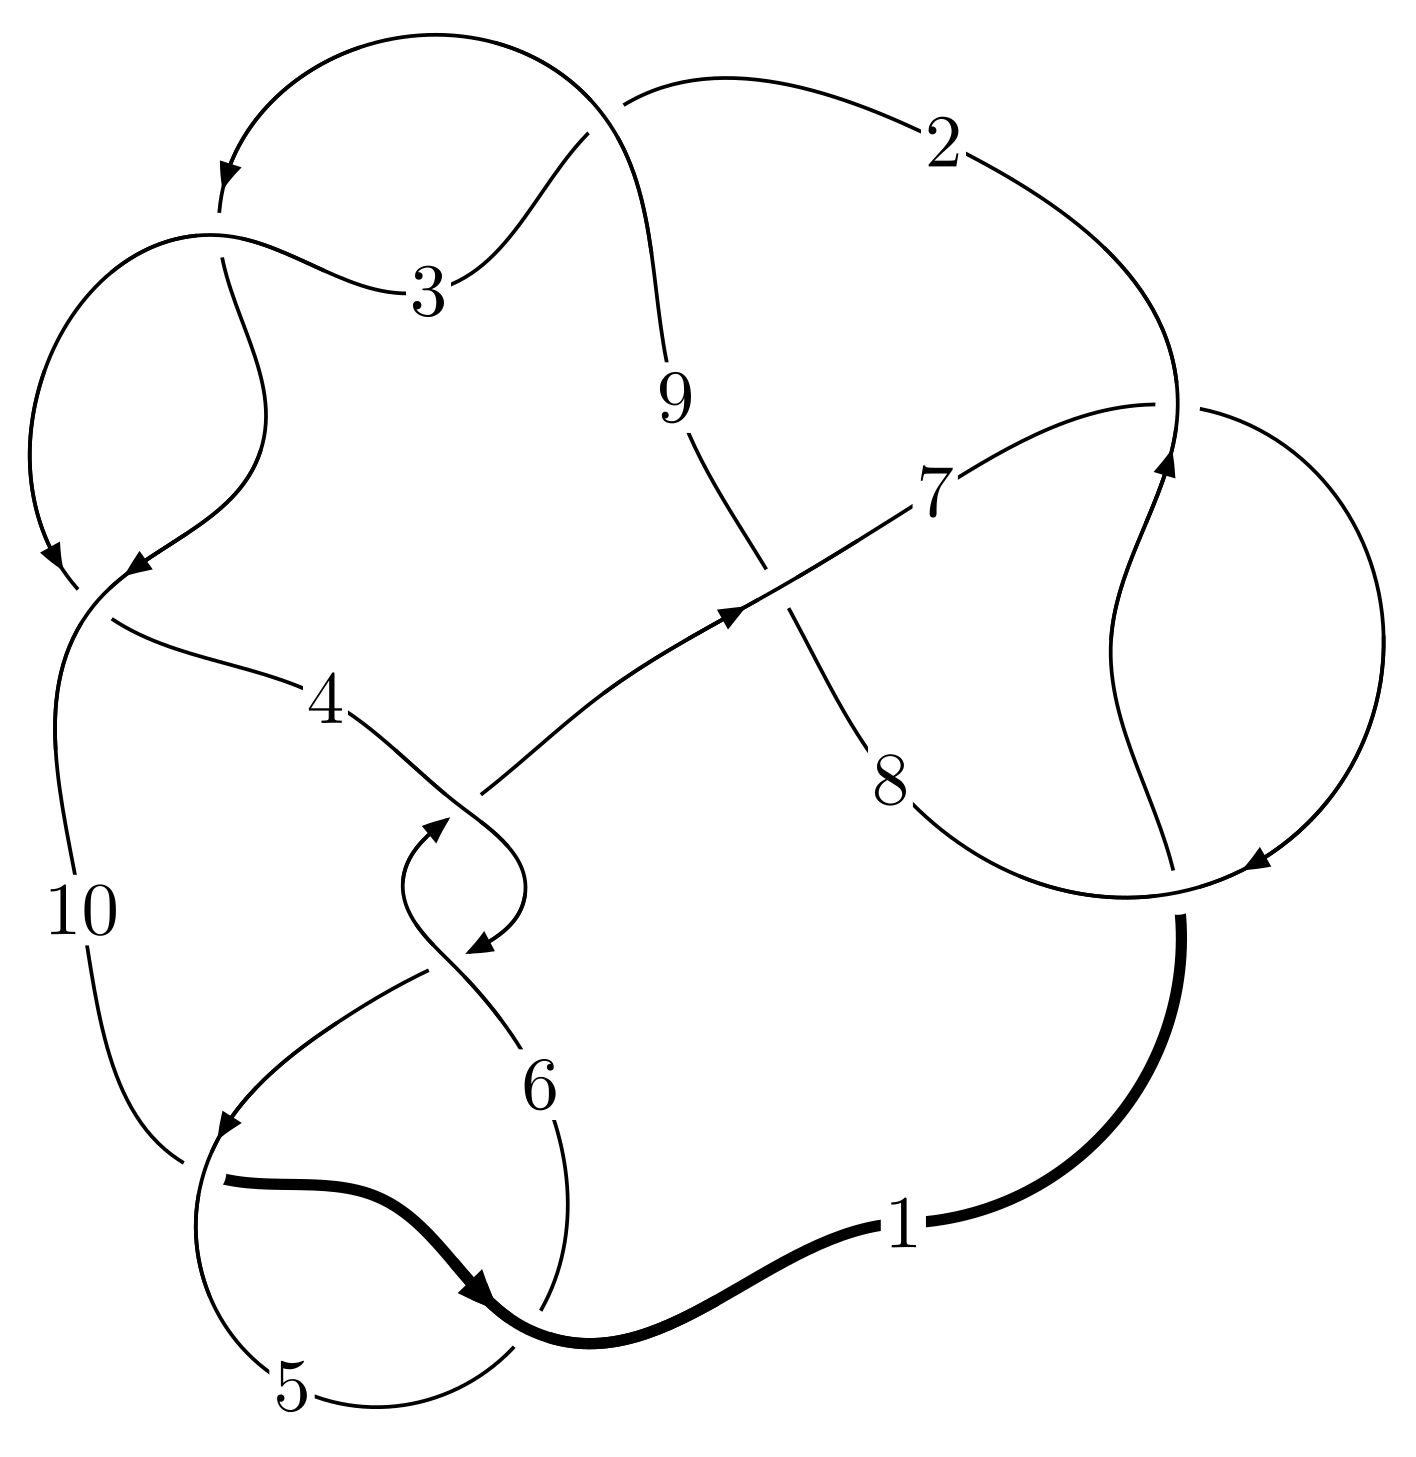
\includegraphics[width=112pt]{../../../GIT/diagram.site/Diagrams/png/123_10_39.png}\\
\ \ \ A knot diagram\footnotemark}&
\allowdisplaybreaks
\textbf{Linearized knot diagam} \\
\cline{2-2}
 &
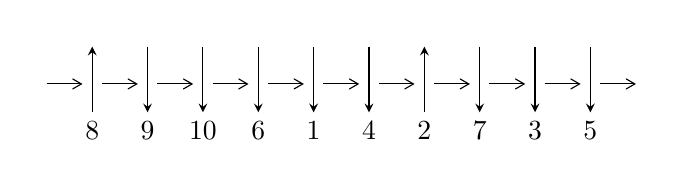
\begin{tikzpicture}[x=20pt, y=17pt]
	% nodes
	\node (C0) at (0, 0) {};
	\node (C1) at (1, 0) {};
	\node (C1U) at (1, +1) {};
	\node (C1D) at (1, -1) {8};

	\node (C2) at (2, 0) {};
	\node (C2U) at (2, +1) {};
	\node (C2D) at (2, -1) {9};

	\node (C3) at (3, 0) {};
	\node (C3U) at (3, +1) {};
	\node (C3D) at (3, -1) {10};

	\node (C4) at (4, 0) {};
	\node (C4U) at (4, +1) {};
	\node (C4D) at (4, -1) {6};

	\node (C5) at (5, 0) {};
	\node (C5U) at (5, +1) {};
	\node (C5D) at (5, -1) {1};

	\node (C6) at (6, 0) {};
	\node (C6U) at (6, +1) {};
	\node (C6D) at (6, -1) {4};

	\node (C7) at (7, 0) {};
	\node (C7U) at (7, +1) {};
	\node (C7D) at (7, -1) {2};

	\node (C8) at (8, 0) {};
	\node (C8U) at (8, +1) {};
	\node (C8D) at (8, -1) {7};

	\node (C9) at (9, 0) {};
	\node (C9U) at (9, +1) {};
	\node (C9D) at (9, -1) {3};

	\node (C10) at (10, 0) {};
	\node (C10U) at (10, +1) {};
	\node (C10D) at (10, -1) {5};
	\node (C11) at (11, 0) {};

	% arrows
	\draw[->,>={angle 60}]
	(C0) edge (C1) (C1) edge (C2) (C2) edge (C3) (C3) edge (C4) (C4) edge (C5) (C5) edge (C6) (C6) edge (C7) (C7) edge (C8) (C8) edge (C9) (C9) edge (C10) (C10) edge (C11) ;	\draw[->,>=stealth]
	(C1D) edge (C1U) (C2U) edge (C2D) (C3U) edge (C3D) (C4U) edge (C4D) (C5U) edge (C5D) (C6U) edge (C6D) (C7D) edge (C7U) (C8U) edge (C8D) (C9U) edge (C9D) (C10U) edge (C10D) ;
	\end{tikzpicture} \\
\hhline{~~} \\& 
\textbf{Solving Sequence} \\ \cline{2-2} 
 &
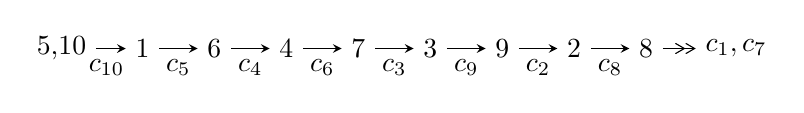
\begin{tikzpicture}[x=26pt, y=7pt]
	% node
	\node (A0) at (-1/8, 0) {5,10};
	\node (A1) at (1, 0) {1};
	\node (A2) at (2, 0) {6};
	\node (A3) at (3, 0) {4};
	\node (A4) at (4, 0) {7};
	\node (A5) at (5, 0) {3};
	\node (A6) at (6, 0) {9};
	\node (A7) at (7, 0) {2};
	\node (A8) at (8, 0) {8};
	\node (C1) at (1/2, -1) {$c_{10}$};
	\node (C2) at (3/2, -1) {$c_{5}$};
	\node (C3) at (5/2, -1) {$c_{4}$};
	\node (C4) at (7/2, -1) {$c_{6}$};
	\node (C5) at (9/2, -1) {$c_{3}$};
	\node (C6) at (11/2, -1) {$c_{9}$};
	\node (C7) at (13/2, -1) {$c_{2}$};
	\node (C8) at (15/2, -1) {$c_{8}$};
	\node (A9) at (37/4, 0) {$c_{1},c_{7}$};

	% edge
	\draw[->,>=stealth]	
	(A0) edge (A1) (A1) edge (A2) (A2) edge (A3) (A3) edge (A4) (A4) edge (A5) (A5) edge (A6) (A6) edge (A7) (A7) edge (A8) ;
	\draw[->>,>={angle 60}]	
	(A8) edge (A9);
\end{tikzpicture} \\ 

\end{tabular} \\

\footnotetext{
The image of knot diagram is generated by the software ``\textbf{Draw programme}" developed by Andrew Bartholomew(\url{http://www.layer8.co.uk/maths/draw/index.htm\#Running-draw}), where we modified some parts for our purpose(\url{https://github.com/CATsTAILs/LinksPainter}).
}\phantom \\ \newline 
\centering \textbf{Ideals for irreducible components\footnotemark of $X_{\text{par}}$} 
 
\begin{align*}
I^u_{1}&=\langle 
u^{30}- u^{29}+\cdots- u-1\rangle \\
\\
\end{align*}
\raggedright * 1 irreducible components of $\dim_{\mathbb{C}}=0$, with total 30 representations.\\
\footnotetext{All coefficients of polynomials are rational numbers. But the coefficients are sometimes approximated in decimal forms when there is not enough margin.}
\newpage
\renewcommand{\arraystretch}{1}
\centering \section*{I. $I^u_{1}= \langle u^{30}- u^{29}+\cdots- u-1 \rangle$}
\flushleft \textbf{(i) Arc colorings}\\
\begin{tabular}{m{7pt} m{180pt} m{7pt} m{180pt} }
\flushright $a_{5}=$&$\begin{pmatrix}0\\u\end{pmatrix}$ \\
\flushright $a_{10}=$&$\begin{pmatrix}1\\0\end{pmatrix}$ \\
\flushright $a_{1}=$&$\begin{pmatrix}1\\u^2\end{pmatrix}$ \\
\flushright $a_{6}=$&$\begin{pmatrix}- u\\- u^3+u\end{pmatrix}$ \\
\flushright $a_{4}=$&$\begin{pmatrix}u^3\\u^5- u^3+u\end{pmatrix}$ \\
\flushright $a_{7}=$&$\begin{pmatrix}- u^5- u\\- u^7+u^5-2 u^3+u\end{pmatrix}$ \\
\flushright $a_{3}=$&$\begin{pmatrix}u^5+u\\u^5- u^3+u\end{pmatrix}$ \\
\flushright $a_{9}=$&$\begin{pmatrix}- u^{10}+u^8-2 u^6+u^4- u^2+1\\- u^{10}+2 u^8-3 u^6+2 u^4- u^2\end{pmatrix}$ \\
\flushright $a_{2}=$&$\begin{pmatrix}- u^{15}+2 u^{13}-4 u^{11}+4 u^9-4 u^7+4 u^5-2 u^3+2 u\\- u^{15}+3 u^{13}-6 u^{11}+7 u^9-6 u^7+4 u^5-2 u^3+u\end{pmatrix}$ \\
\flushright $a_{8}=$&$\begin{pmatrix}u^{22}-3 u^{20}+\cdots-3 u^4+1\\u^{24}-4 u^{22}+\cdots+8 u^4-2 u^2\end{pmatrix}$\\&\end{tabular}
\flushleft \textbf{(ii) Obstruction class $= -1$}\\~\\
\flushleft \textbf{(iii) Cusp Shapes $= -4 u^{28}+20 u^{26}-4 u^{25}-64 u^{24}+16 u^{23}+140 u^{22}-48 u^{21}-236 u^{20}+96 u^{19}+320 u^{18}-156 u^{17}-356 u^{16}+208 u^{15}+340 u^{14}-228 u^{13}-272 u^{12}+220 u^{11}+188 u^{10}-168 u^9-108 u^8+116 u^7+48 u^6-64 u^5-20 u^4+28 u^3+4 u^2-8 u-10$}\\~\\
\newpage\renewcommand{\arraystretch}{1}
\flushleft \textbf{(iv) u-Polynomials at the component}\newline \\
\begin{tabular}{m{50pt}|m{274pt}}
Crossings & \hspace{64pt}u-Polynomials at each crossing \\
\hline $$\begin{aligned}c_{1},c_{7}\end{aligned}$$&$\begin{aligned}
&u^{30}- u^{29}+\cdots- u-1
\end{aligned}$\\
\hline $$\begin{aligned}c_{2},c_{3},c_{9}\end{aligned}$$&$\begin{aligned}
&u^{30}+u^{29}+\cdots+7 u-1
\end{aligned}$\\
\hline $$\begin{aligned}c_{4},c_{6}\end{aligned}$$&$\begin{aligned}
&u^{30}+11 u^{29}+\cdots+u+1
\end{aligned}$\\
\hline $$\begin{aligned}c_{5},c_{10}\end{aligned}$$&$\begin{aligned}
&u^{30}- u^{29}+\cdots- u-1
\end{aligned}$\\
\hline $$\begin{aligned}c_{8}\end{aligned}$$&$\begin{aligned}
&u^{30}+17 u^{29}+\cdots- u+1
\end{aligned}$\\
\hline
\end{tabular}\\~\\
\newpage\renewcommand{\arraystretch}{1}
\flushleft \textbf{(v) Riley Polynomials at the component}\newline \\
\begin{tabular}{m{50pt}|m{274pt}}
Crossings & \hspace{64pt}Riley Polynomials at each crossing \\
\hline $$\begin{aligned}c_{1},c_{7}\end{aligned}$$&$\begin{aligned}
&y^{30}+17 y^{29}+\cdots- y+1
\end{aligned}$\\
\hline $$\begin{aligned}c_{2},c_{3},c_{9}\end{aligned}$$&$\begin{aligned}
&y^{30}-31 y^{29}+\cdots-49 y+1
\end{aligned}$\\
\hline $$\begin{aligned}c_{4},c_{6}\end{aligned}$$&$\begin{aligned}
&y^{30}+17 y^{29}+\cdots+7 y+1
\end{aligned}$\\
\hline $$\begin{aligned}c_{5},c_{10}\end{aligned}$$&$\begin{aligned}
&y^{30}-11 y^{29}+\cdots- y+1
\end{aligned}$\\
\hline $$\begin{aligned}c_{8}\end{aligned}$$&$\begin{aligned}
&y^{30}-7 y^{29}+\cdots-25 y+1
\end{aligned}$\\
\hline
\end{tabular}\\~\\
\newpage\flushleft \textbf{(vi) Complex Volumes and Cusp Shapes}
$$\begin{array}{c|c|c}  
\text{Solutions to }I^u_{1}& \I (\text{vol} + \sqrt{-1}CS) & \text{Cusp shape}\\
 \hline 
\begin{aligned}
u &= -0.730327 + 0.712584 I\end{aligned}
 & \phantom{-}1.67645 - 2.06909 I & -4.15841 + 3.38718 I \\ \hline\begin{aligned}
u &= -0.730327 - 0.712584 I\end{aligned}
 & \phantom{-}1.67645 + 2.06909 I & -4.15841 - 3.38718 I \\ \hline\begin{aligned}
u &= \phantom{-}0.551518 + 0.799916 I\end{aligned}
 & -5.35554 + 6.07028 I & -8.34155 - 3.40396 I \\ \hline\begin{aligned}
u &= \phantom{-}0.551518 - 0.799916 I\end{aligned}
 & -5.35554 - 6.07028 I & -8.34155 + 3.40396 I \\ \hline\begin{aligned}
u &= -0.906793 + 0.533130 I\end{aligned}
 & -1.75153 + 2.04857 I & -11.94351 - 2.92796 I \\ \hline\begin{aligned}
u &= -0.906793 - 0.533130 I\end{aligned}
 & -1.75153 - 2.04857 I & -11.94351 + 2.92796 I \\ \hline\begin{aligned}
u &= \phantom{-}0.804216 + 0.685158 I\end{aligned}
 & \phantom{-}2.71504 - 2.05267 I & -1.58203 + 3.48780 I \\ \hline\begin{aligned}
u &= \phantom{-}0.804216 - 0.685158 I\end{aligned}
 & \phantom{-}2.71504 + 2.05267 I & -1.58203 - 3.48780 I \\ \hline\begin{aligned}
u &= \phantom{-}0.924638 + 0.148092 I\end{aligned}
 & -3.63670 - 2.97945 I & -13.9208 + 5.3409 I \\ \hline\begin{aligned}
u &= \phantom{-}0.924638 - 0.148092 I\end{aligned}
 & -3.63670 + 2.97945 I & -13.9208 - 5.3409 I \\ \hline\begin{aligned}
u &= -0.543400 + 0.758728 I\end{aligned}
 & -1.94581 - 1.35458 I & -5.23413 + 0.23076 I \\ \hline\begin{aligned}
u &= -0.543400 - 0.758728 I\end{aligned}
 & -1.94581 + 1.35458 I & -5.23413 - 0.23076 I \\ \hline\begin{aligned}
u &= \phantom{-}0.488569 + 0.765822 I\end{aligned}
 & -5.74978 - 2.99724 I & -8.94829 + 3.11480 I \\ \hline\begin{aligned}
u &= \phantom{-}0.488569 - 0.765822 I\end{aligned}
 & -5.74978 + 2.99724 I & -8.94829 - 3.11480 I \\ \hline\begin{aligned}
u &= \phantom{-}0.897290 + 0.672452 I\end{aligned}
 & \phantom{-}2.42981 - 3.18388 I & -2.48294 + 3.33039 I \\ \hline\begin{aligned}
u &= \phantom{-}0.897290 - 0.672452 I\end{aligned}
 & \phantom{-}2.42981 + 3.18388 I & -2.48294 - 3.33039 I \\ \hline\begin{aligned}
u &= \phantom{-}1.12154\phantom{ +0.000000I}\end{aligned}
 & -7.57426\phantom{ +0.000000I} & -11.4920\phantom{ +0.000000I} \\ \hline\begin{aligned}
u &= -1.139570 + 0.022635 I\end{aligned}
 & -11.30750 + 4.69703 I & -14.6642 - 3.2976 I \\ \hline\begin{aligned}
u &= -1.139570 - 0.022635 I\end{aligned}
 & -11.30750 - 4.69703 I & -14.6642 + 3.2976 I \\ \hline\begin{aligned}
u &= -0.950905 + 0.682953 I\end{aligned}
 & \phantom{-}1.01456 + 7.42449 I & -6.02063 - 8.82247 I \\ \hline\begin{aligned}
u &= -0.950905 - 0.682953 I\end{aligned}
 & \phantom{-}1.01456 - 7.42449 I & -6.02063 + 8.82247 I \\ \hline\begin{aligned}
u &= -1.047270 + 0.654174 I\end{aligned}
 & -3.41555 + 6.72016 I & -7.40084 - 4.93754 I \\ \hline\begin{aligned}
u &= -1.047270 - 0.654174 I\end{aligned}
 & -3.41555 - 6.72016 I & -7.40084 + 4.93754 I \\ \hline\begin{aligned}
u &= \phantom{-}1.060070 + 0.635598 I\end{aligned}
 & -7.40758 - 2.28828 I & -11.38974 + 1.78470 I \\ \hline\begin{aligned}
u &= \phantom{-}1.060070 - 0.635598 I\end{aligned}
 & -7.40758 + 2.28828 I & -11.38974 - 1.78470 I \\ \hline\begin{aligned}
u &= \phantom{-}1.059080 + 0.667496 I\end{aligned}
 & -6.86248 - 11.58950 I & -10.39391 + 7.89908 I \\ \hline\begin{aligned}
u &= \phantom{-}1.059080 - 0.667496 I\end{aligned}
 & -6.86248 + 11.58950 I & -10.39391 - 7.89908 I \\ \hline\begin{aligned}
u &= -0.704437\phantom{ +0.000000I}\end{aligned}
 & -1.05262\phantom{ +0.000000I} & -9.30020\phantom{ +0.000000I} \\ \hline\begin{aligned}
u &= -0.175683 + 0.414203 I\end{aligned}
 & -0.50312 + 1.32269 I & -5.12281 - 4.79072 I \\ \hline\begin{aligned}
u &= -0.175683 - 0.414203 I\end{aligned}
 & -0.50312 - 1.32269 I & -5.12281 + 4.79072 I\\
 \hline 
 \end{array}$$\newpage
\newpage\renewcommand{\arraystretch}{1}
\centering \section*{ II. u-Polynomials}
\begin{tabular}{m{50pt}|m{274pt}}
Crossings & \hspace{64pt}u-Polynomials at each crossing \\
\hline $$\begin{aligned}c_{1},c_{7}\end{aligned}$$&$\begin{aligned}
&u^{30}- u^{29}+\cdots- u-1
\end{aligned}$\\
\hline $$\begin{aligned}c_{2},c_{3},c_{9}\end{aligned}$$&$\begin{aligned}
&u^{30}+u^{29}+\cdots+7 u-1
\end{aligned}$\\
\hline $$\begin{aligned}c_{4},c_{6}\end{aligned}$$&$\begin{aligned}
&u^{30}+11 u^{29}+\cdots+u+1
\end{aligned}$\\
\hline $$\begin{aligned}c_{5},c_{10}\end{aligned}$$&$\begin{aligned}
&u^{30}- u^{29}+\cdots- u-1
\end{aligned}$\\
\hline $$\begin{aligned}c_{8}\end{aligned}$$&$\begin{aligned}
&u^{30}+17 u^{29}+\cdots- u+1
\end{aligned}$\\
\hline
\end{tabular}\newpage\renewcommand{\arraystretch}{1}
\centering \section*{ III. Riley Polynomials}
\begin{tabular}{m{50pt}|m{274pt}}
Crossings & \hspace{64pt}Riley Polynomials at each crossing \\
\hline $$\begin{aligned}c_{1},c_{7}\end{aligned}$$&$\begin{aligned}
&y^{30}+17 y^{29}+\cdots- y+1
\end{aligned}$\\
\hline $$\begin{aligned}c_{2},c_{3},c_{9}\end{aligned}$$&$\begin{aligned}
&y^{30}-31 y^{29}+\cdots-49 y+1
\end{aligned}$\\
\hline $$\begin{aligned}c_{4},c_{6}\end{aligned}$$&$\begin{aligned}
&y^{30}+17 y^{29}+\cdots+7 y+1
\end{aligned}$\\
\hline $$\begin{aligned}c_{5},c_{10}\end{aligned}$$&$\begin{aligned}
&y^{30}-11 y^{29}+\cdots- y+1
\end{aligned}$\\
\hline $$\begin{aligned}c_{8}\end{aligned}$$&$\begin{aligned}
&y^{30}-7 y^{29}+\cdots-25 y+1
\end{aligned}$\\
\hline
\end{tabular}
\vskip 2pc
\end{document}